\chapter{Theoretical concepts}


\section*{Common type of aircraft's structures}
\noindent
The structures of aircrafts have significantly changed during time and advances in materials and processes used to construct the fuselage have led to their evolution from simple wood truss structures to the sleek composite and aerodynamic flying machines of today. \\
Despite the wide variety of different shapes and geometries existing, three common basic types of structures can be highlighted at the base of aircraft's design: 
\begin{itemize}
	\item TRUSS TYPE (or tubular);
	\item MONOCOQUE / SEMI-MONOCOQUE (or stress-skin);
	\item BONDED (or composite construction).
\end{itemize}  


\noindent A brief general description of the main features of these kinds of structures is now outlined for completeness.
\smallskip
\noindent 
\subsubsection*{TRUSS TYPE (or tubular)}
\addcontentsline{toc}{section}{Truss structures}
\noindent This type of construction is typical of the early generation of airplanes and it is still in use in many lightweight aicrafts and helicopters. It is quite simple and it consists typically in \emph{welded steel tube trusses} which form a rigid frame in such a manner that all members
of the truss can carry both tension and compression loads. \\ 

\smallskip
\noindent 
\emph{Advantages}: 
\begin{itemize}
	\item High strenght to weight ratio;
	\item Simple; can be repaired at field level unless need for a jig for alignment process.
\end{itemize}


\smallskip
\noindent 
\emph{Disadvantages}: \begin{itemize}
	\item High costs of manufacturing;
	\item Difficult to hold dimensions to a close tolerance.
\end{itemize}

\smallskip
\noindent 
Normally it consists in 3 or 4 \underline{longerons} that run the entire structure's length; they took most of the compressive and tensile loads and resists to the flexural deformation. \\
Longeron are kept apart by \underline{cross members} (ideally subject only in tension / compression) which can be arranged in different configurations eg. 'N', 'X' oe 'W' to cope with the side ways loads (e.g. tail rotor thrust in helicopters). \\
\underline{Diagonal members} (or cross bracing) took the internal space and complete the structure. \\
In some aircraft, principally the light, single engine
models, truss fuselage frames may be constructed of
aluminum alloy and may be riveted or bolted into one piece,
with cross-bracing achieved by using solid rods or tubes. \\

\noindent


\smallskip
\begin{figure}[h!]
	\begin{center}
		\centering  		 		
		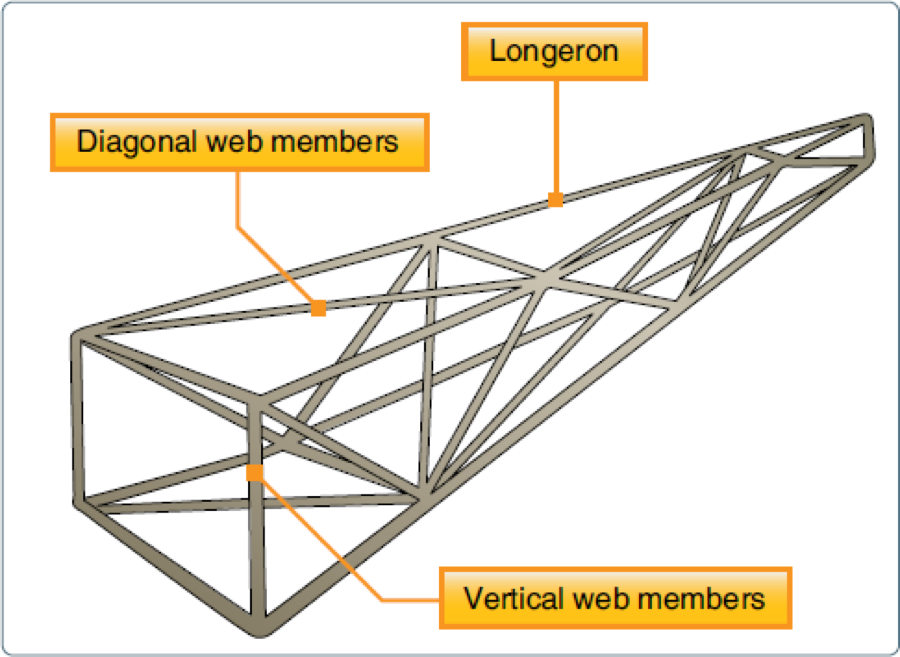
\includegraphics[width=0.7\linewidth]{PICTURES/1_Theory/PNG/truss_members.png}
	\end{center}
	\caption {Example of a Warren truss structure}
\end{figure}
%\vspace{0.5cm}



\clearpage
\noindent 
\subsubsection*{SEMI-MONOCOQUE CONSTRUCTION}
\addcontentsline{toc}{section}{Semi-monocoque construction}
\noindent This is the preferred method of constructing aluminium fuselages and can be either MONOCOQUE or SEMI-MONOCOQUE depending on the role of the outer skin. In the first case the exterior surface of the fuselage is also a primary structure so it contributes to resist external loads while in the second case it is just a coverage and helps only to resist to torsions. \\
The biggest problem involved in monocoque constructions is maintaining enough strength while keeping the weight within allowable limits. This problem is typically overcome using semi-monocoque constructions. \\
These kinds of structures consist of a series of \underline{vertical frames} in the shape of the fuselage's cross sections held in position on a rigid fixture, or jig and joined together with \underline{longerons} (typically made of aluminum alloys) which extend across several frame members and help the skin to support primary bending loads. Also lightweight longitudinal elements called \underline{stringers} can be used to further reinforcement which are typically more numerous and lighter in weight than the longerons. All these elements are in turn covered with a skin of sheet aluminium, attached by riveting. 
Most modern aircraft are considered to be of semi-monocoque type construction. \\

\smallskip
\begin{figure}[h!]
	\begin{center}
		\centering  		 		
		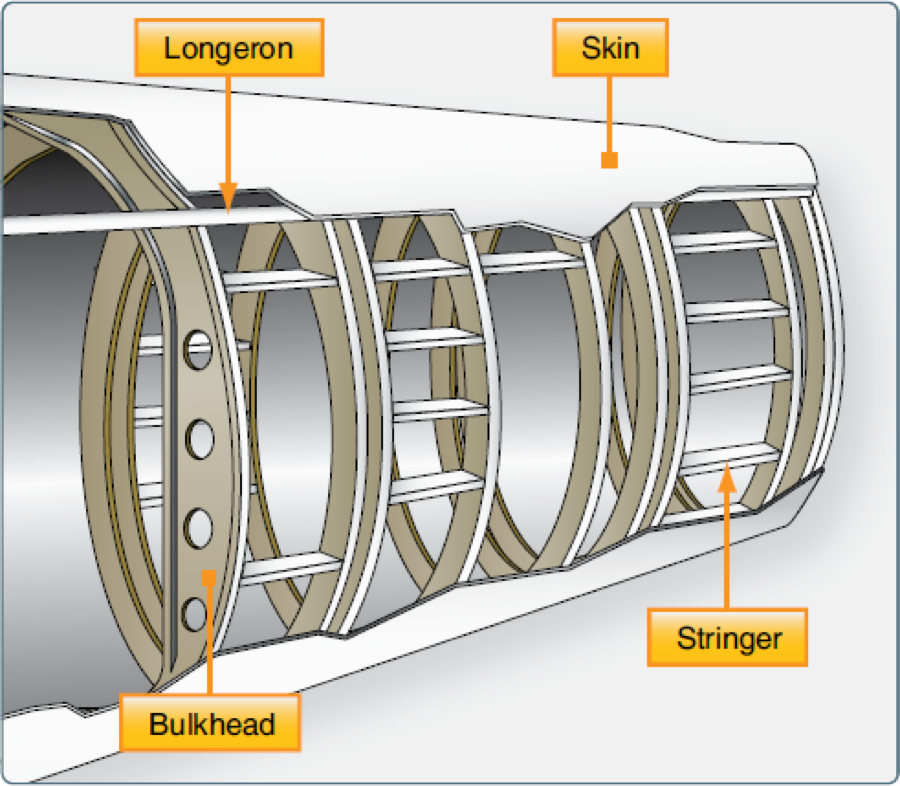
\includegraphics[width=0.7\linewidth]{PICTURES/1_Theory/PNG/semi-monocoque.png}
	\end{center}
	\caption {The most common airframe construction (semi-monocoque).}
\end{figure}
%\vspace{0.5cm}

\noindent 
The semimonocoque fuselage is constructed primarily of alloys of aluminum and magnesium, although steel and titanium are sometimes found in areas of high temperatures. \\ The fuselage skin thickness can vary with the
load carried and the stresses sustained at a particular location. \\

\smallskip
\noindent 
\emph{Advantages}: \begin{itemize}
	\item High strenght to weight ratio (higher than the truss constructions of the same size);
	\item Spreading loads among different structures and
	the skin means no single piece is failure critical;
	\item Easy to manufacture and faster;
	\item More precision in terms of fitting tolerances.
\end{itemize}

\bigskip
\noindent
 \subsubsection*{BONDED CONSTRUCTION}
 
\noindent The third type of construction involves structure whose parts are joined together by chemical methods rather than mechanical.\\ Fibreglass, honeycomb and other composite materials are used in these structures by the use of adhesives, glues, heat and pressure. \\

\smallskip
\noindent
\emph{Advantage}:
 \begin{itemize}
	\item High strenght to weight ratios, reduced construction cost by eliminating riveting and welding.
\end{itemize}



